\documentclass[11pt]{article}

\usepackage{times}
\usepackage{epsf}
\usepackage{epsfig}
\usepackage{amsmath, alltt, amssymb, xspace}
\usepackage{wrapfig}
\usepackage{fancyhdr}
\usepackage{url}
\usepackage{verbatim}
\usepackage{fancyvrb}
\usepackage{float}

\usepackage{subfigure}
\usepackage{cite}
\usepackage{hyperref}
\hypersetup{%
    pdfborder = {0 0 0}
}
\topmargin      -0.50in  % distance to headers
\oddsidemargin  0.0in
\evensidemargin 0.0in
\textwidth      6.5in
\textheight     8.9in 


%\centerfigcaptionstrue

%\def\baselinestretch{0.95}


\newcommand\discuss[1]{\{\textbf{Discuss:} \textit{#1}\}}
%\newcommand\todo[1]{\vspace{0.1in}\{\textbf{Todo:} \textit{#1}\}\vspace{0.1in}}
\newtheorem{problem}{Problem}[section]
%\newtheorem{theorem}{Theorem}
%\newtheorem{fact}{Fact}
\newtheorem{define}{Definition}[section]
%\newtheorem{analysis}{Analysis}
\newcommand\vspacenoindent{\vspace{0.1in} \noindent}

%\newenvironment{proof}{\noindent {\bf Proof}.}{\hspace*{\fill}~\mbox{\rule[0pt]{1.3ex}{1.3ex}}}
%\newcommand\todo[1]{\vspace{0.1in}\{\textbf{Todo:} \textit{#1}\}\vspace{0.1in}}

%\newcommand\reducespace{\vspace{-0.1in}}
% reduce the space between lines
%\def\baselinestretch{0.95}

\newcommand{\fixmefn}[1]{ \footnote{\sf\ \ \fbox{FIXME} #1} }
\newcommand{\todo}[1]{
\vspace{0.1in}
\fbox{\parbox{6in}{TODO: #1}}
\vspace{0.1in}
}

\newcommand{\mybox}[1]{
\vspace{0.2in}
\noindent
\fbox{\parbox{6.5in}{#1}}
\vspace{0.1in}
}


\newcounter{question}
\setcounter{question}{1}

\newcommand{\myquestion} {{\vspace{0.1in} \noindent \bf Question \arabic{question}:} \addtocounter{question}{1} \,}

\newcommand{\myproblem} {{\noindent \bf Problem \arabic{question}:} \addtocounter{question}{1} \,}


\newcommand{\copyrightnotice}[1]{
\vspace{0.1in}
\fbox{\parbox{6in}{
      This lab was developed for the Labtainer framework by the Naval Postgraduate
      School, Center for Cybersecurity and Cyber Operations under sponsorship from
      the DoD CySP program.  This work is in the public domain, and cannot be copyrighted.}}
\vspace{0.1in}
}


\newcommand{\idea}[1]{
\vspace{0.1in}
{\sf IDEA:\ \ \fbox{\parbox{5in}{#1}}}
\vspace{0.1in}
}

\newcommand{\questionblock}[1]{
\vspace{0.1in}
\fbox{\parbox{6in}{#1}}
\vspace{0.1in}
}


\newcommand{\argmax}[1]{
\begin{minipage}[t]{1.25cm}\parskip-1ex\begin{center}
argmax
#1
\end{center}\end{minipage}
\;
}

\newcommand{\bm}{\boldmath}
\newcommand  {\bx}    {\mbox{\boldmath $x$}}
\newcommand  {\by}    {\mbox{\boldmath $y$}}
\newcommand  {\br}    {\mbox{\boldmath $r$}}


\newcommand{\tstamp}{\today}   
%\rfoot[\fancyplain{\tstamp} {\tstamp}]  {\fancyplain{}{}}

\pagestyle{fancy}
\lhead{\bfseries Labtainers}
\chead{}
\rhead{\small \thepage}
\lfoot{}
\cfoot{}
\rfoot{}




\begin{document}

\begin{center}
{\LARGE IPTABLES}
\vspace{0.1in}\\
\end{center}


\section{Overview}
This Labtainer exercise illustrates the use of iptables
on a firewall to limit network access to a server from a client,
as illustrated in figure 
\ref{fig:topology}

When properly configured, the firewall will only allow selected
traffic from the client to the server.

\subsection {Background}
Limiting the types of network traffic sent to a server can help to
protect the server from unauthorized access.  For example, if the
server contains an unsecured service available through its network
interface, exploitation of that service is more difficult if something
blocks traffic destined for that service.

A variety of different techniques and products exist for the purpose of limiting
IP network traffic between computers.  In this lab, you will limit IP traffic through
use of Linux iptables.  
The student is expected to have separately learned about the use of iptables
to selectively block network traffic. The firewall component includes an
example firewall setting script that you can reference.  The manpage for iptables can be viewed on the
firewall component using:
\begin{verbatim}
   man iptables
   man iptables-extensions
\end{verbatim}

Students are expected to have a basic 
familiarity with the Linux command line, and the ability to edit files and
run simple shell scripts. Some experience with Wireshark is presumed, e.g., performance of
the wireshark-intro lab.

\section{Lab Environment}
This lab runs in the Labtainer framework,
available at http://nps.edu/web/c3o/labtainers.
That site includes links to a pre-built virtual machine
that has Labtainers installed, however Labtainers can
be run on any Linux host that supports Docker containers.

From your labtainer-student directory start the lab using:
\begin{verbatim}
    labtainer iptables2
\end{verbatim}
\noindent A link to this lab manual will be displayed.  


\begin{figure}[H]
\begin{center}
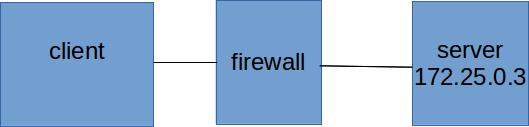
\includegraphics [width=0.8\textwidth]{iptables.jpg}
\end{center}
\caption{Network topology for the iptables lab}
\label{fig:topology}
\end{figure}

\section{Lab Tasks}
\subsection{Prep quiz}
Take a quick quiz to confirm you are prepared to perform the lab.
At the terminal from which you started the lab, type: 
\begin{verbatim}
   quiz
\end{verbatim}
\subsection{Explore}
\begin{itemize}
\item The Wireshark utility is installed on the firewall. 
Use it to view network traffic through the firewall, and to 
debug your firewall rules.  Start it from the firewall terminal:
\begin{verbatim}
wireshark &
\end{verbatim}
\noindent Then select the eth0 interface.

\item On the client terminal use the nmap utility 
to list (some of the) open ports on the server:

\begin{verbatim}
        nmap server
\end{verbatim}

\item Use wget to confirm that the server response to HTTP requests:
\begin{verbatim}
        wget server &
\end{verbatim}
\item Confirm an ssh service if offered -- you need not login when prompted,
just use {\tt ctrl C} to exit once you get a response from the server.
\begin{verbatim}
        ssh server
\end{verbatim}
\item Finally, confirm that telnet is offered (again, no need to login):
\begin{verbatim}
        telnet server
\end{verbatim}
\item Observe the traffic in wireshark, making note the
source IP addresses and the destination ports used by the 
clients when connecting to the server
\end{itemize}

\subsection{Use iptables to limit traffic}
The iptables utility is installed on the ``firewall'' component.
Use it to prevent the firewall from forwarding any traffic
to the server other than SSH and HTTP.

You may reference and experiment with the example firewall script that
is on the firewall component in the home directory.  
To run the {\tt example\_fw.sh} script, use:
\begin{verbatim}
        sudo ./example_fw.sh
\end{verbatim}
View the content of the script to understand what it does.
Consider putting your iptables commands in a script so it is easy
to test and reconfigure the iptables if you restart the lab.

Note the last line in the {\tt example\_fw.sh} script directs iptables
to log dropped packets.  You can view these from one of the firewall terminal
tabs via:
\begin{verbatim}
        tail -f /var/log/iptables.log
\end{verbatim}

After modifying your iptables configuration, use the applications on the client to
demonstrate that the firewall only allows the desired traffic.
Watch the traffic in wireshark to see that the TCP handshake fails
when attempting to connect to filtered ports.

Use nmap to confirm the proper configuration:
\begin{verbatim}
   nmap server
\end{verbatim}


\subsection{Open new service port}
The client computer includes a {\tt wizbang} program that you must now allow to send
traffic to the server.  Run the program from the client, and observe which port it
attempts to use within wireshark:
\begin{verbatim}
    ./wizbang
\end{verbatim}
\noindent Then alter your iptables to allow this service.  After adjusting your iptables, 
confirm that you can run the {\tt wizbang} program successfully.
Also, again use nmap to confirm the proper configuration
\begin{verbatim}
   nmap server
\end{verbatim}

\subsection{Check your work}
Use the {\tt checkwork} command from the terminal you used to start the lab.  This will
provide feedback indicating whether you have achieved the goals of the lab.

\section{Submission}
After finishing the lab, go to the terminal on your Linux system that was used to start the lab and type:
\begin{verbatim}
    stoplab 
\end{verbatim}
When you stop the lab, the system will display a path to the zipped lab results on your Linux system.  Provide that file to 
your instructor, e.g., via the Sakai site.

\copyrightnotice

\end{document}
